\section{Control Module}

The control module is responsible for coordinating the activity of the
other parts of the image processor and for data transfer into and within
the image processor. A visual overview of the control module is given in
figure \ref{fig:control-module}.

\begin{figure}[h!]
\centering
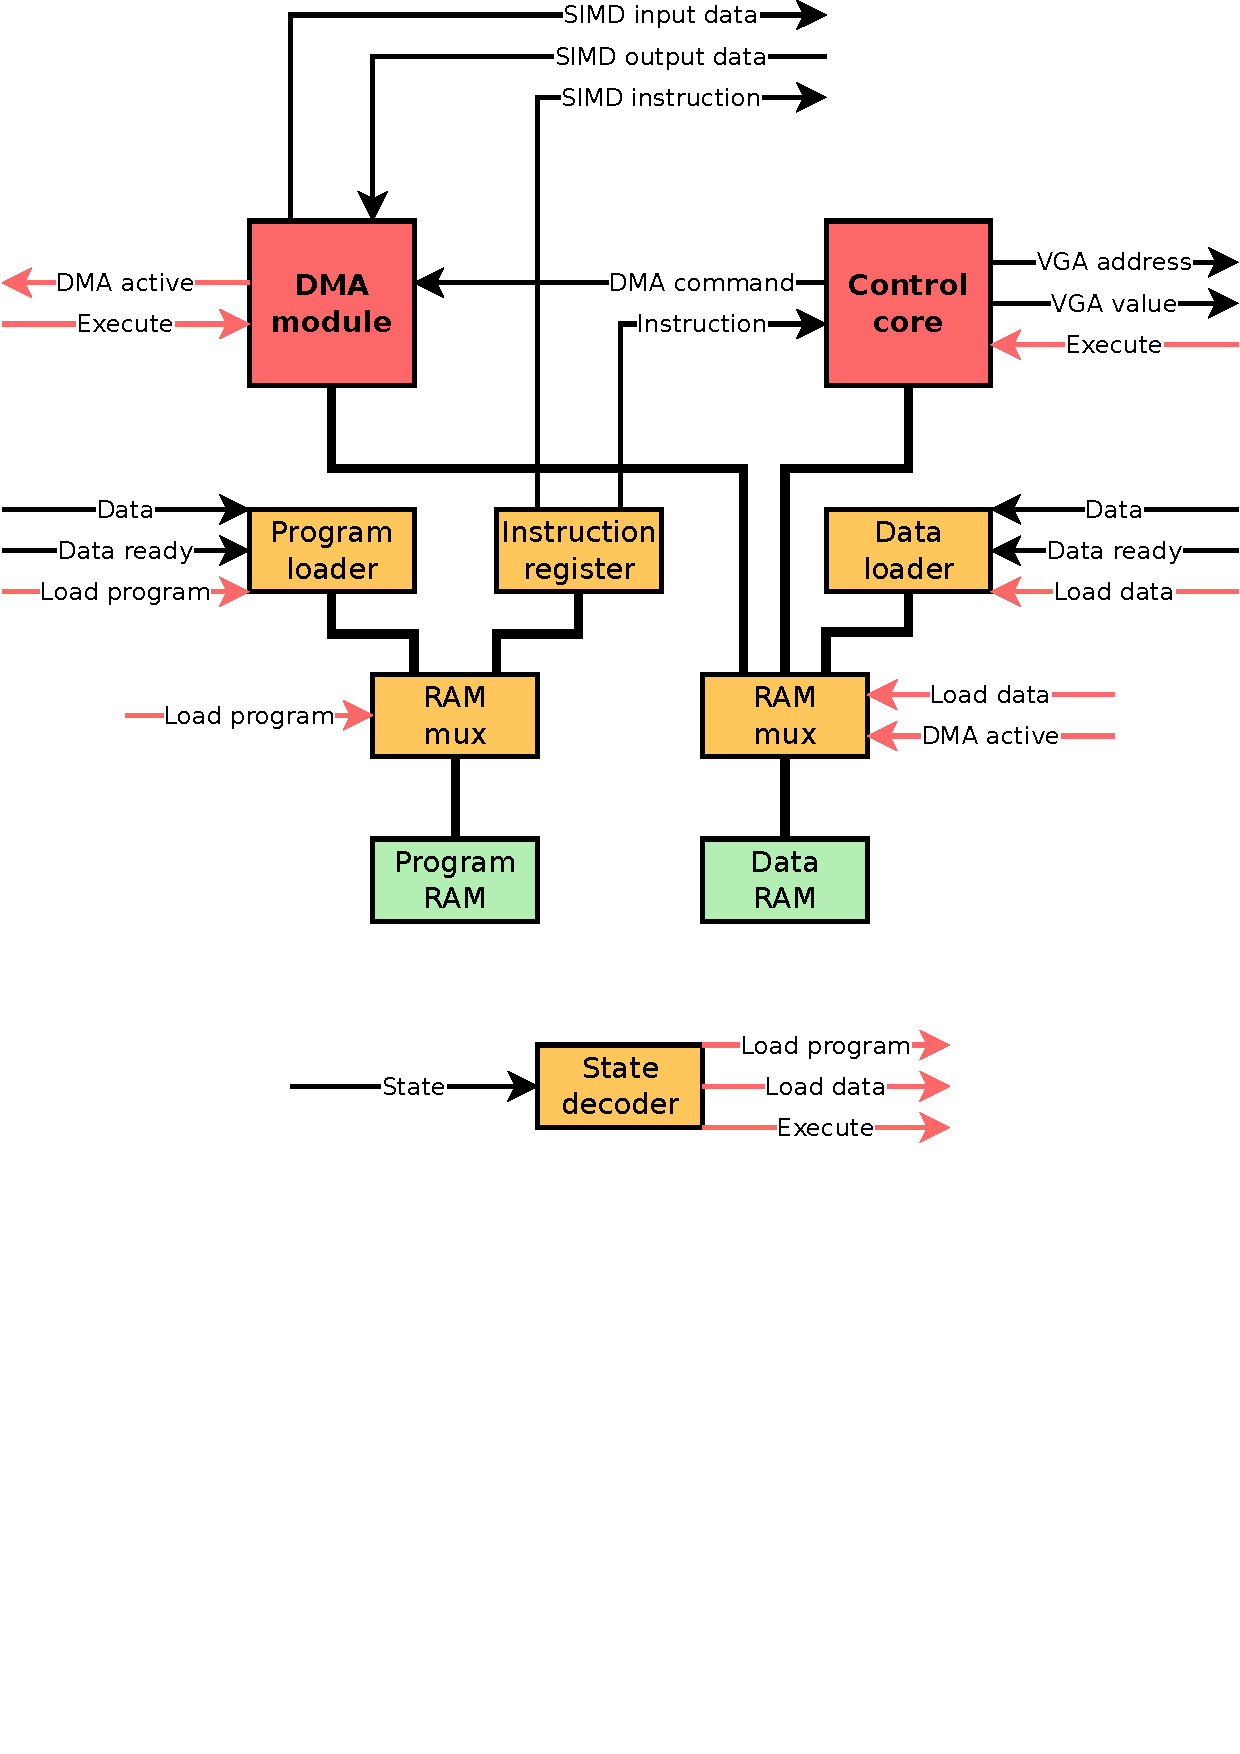
\includegraphics[width=\linewidth,clip,trim=0 10cm 0 0]
                {fig/fpga/control_module.pdf}
\caption[Control module]
        {An overview of the control module of the image processor.}
\label{fig:control-module}
\end{figure}


The control module decodes the state signal set by the AVR, and enables,
disables and resets components accordingly. It is responsible for
performing data transfers between the AVR and the program/data memories,
and for transferring data internally, between the SIMD node array, data
RAM and the VGA screen buffer.

The control module contains the CPU core that is used for the non-SIMD
instructions embedded in a program. This CPU core, henceforth referred
to as the \emph{control core}, is mainly concerned with loop control,
initiating data transfers between the SIMD node array and the data RAM,
and copying image data to the VGA controller.

\subsection{States}

The operation of the image processor is fully controlled by the SCU. The
SCU sets a state value that is used by the control module to select
which components of the image processor are active. This is indicated by
the red signals in figure \ref{fig:control-module}.

The states recognized by the image processor are listed in table
\ref{tab:states}.

\begin{table}[h]
  \centering
  \begin{tabular}{cl}\toprule
    \thx{State} & \thx{Description} \\ \midrule
    000 & Idle \\
    001 & Run program \\
    010 & Load data from SCU \\
    100 & Load program from SCU \\
    \bottomrule
  \end{tabular}
  \caption{Image processor states.}
  \label{tab:states}
\end{table}


\subsection{Control Core}
\subsection{DMA}
\subsection{Program Flow}
